% CVPR 2024 Paper Template; see https://github.com/cvpr-org/author-kit
%\usepackage[inkscapelatex=false]{svg}
\documentclass[10pt,twocolumn,letterpaper]{article}


%%%%%%%%% PAPER TYPE  - PLEASE UPDATE FOR FINAL VERSION
% \usepackage{cvpr}              % To produce the CAMERA-READY version
\usepackage{cvpr}      % To produce the REVIEW version
% \usepackage[pagenumbers]{cvpr} % To force page numbers, e.g. for an arXiv version

% Import additional packages in the preamble file, before hyperref
%
% --- inline annotations
%
\usepackage[dvipsnames]{xcolor}
\newcommand{\red}[1]{{\color{red}#1}}
\newcommand{\todo}[1]{{\color{red}#1}}
\newcommand{\TODO}[1]{\textbf{\color{red}[TODO: #1]}}
% --- disable by uncommenting  
% \renewcommand{\TODO}[1]{}
% \renewcommand{\todo}[1]{#1}


\usepackage{algorithm}
% \usepackage{algorithmic}
\usepackage{algpseudocode}
\usepackage{amsmath}
% \usepackage{float}
% \usepackage{algorithmicx}



% It is strongly recommended to use hyperref, especially for the review version.
% hyperref with option pagebackref eases the reviewers' job.
% Please disable hyperref *only* if you encounter grave issues, 
% e.g. with the file validation for the camera-ready version.
%
% If you comment hyperref and then uncomment it, you should delete *.aux before re-running LaTeX.
% (Or just hit 'q' on the first LaTeX run, let it finish, and you should be clear).
\definecolor{cvprblue}{rgb}{0.21,0.49,0.74}
\usepackage[pagebackref,breaklinks,colorlinks,citecolor=cvprblue]{hyperref}


%%%%%%%%% PAPER ID  - PLEASE UPDATE
\def\paperID{*****} % *** Enter the Paper ID here
\def\confName{CVPR}
\def\confYear{2024}

%%%%%%%%% TITLE - PLEASE UPDATE
\title{Assignment 2: How Hyperparameter Influence the ViT? \\
a Case Study on MobileVit by Hyperparameter Tuning}

%%%%%%%%% AUTHORS - PLEASE UPDATE
\author{Zhengyang li\\
   School of Computer and Mathematical Sciences\\
   Adelaide, South Australia 5005 Australia\\
   \tt\small Zhengyang.li01@adelaide.edu.au}
% For a paper whose authors are all at the same institution,
% omit the following lines up until the closing ``}''.
% Additional authors and addresses can be added with ``\and'',
% just like the second author.
% To save space, use either the email address or home page, not both

\begin{document}
\maketitle

\begin{abstract}
   This study constitutes an in-depth analysis of the pivotal factors that influence the performance of neural network models on the CIFAR-100 dataset, with a focus on multi-head attention mechanisms, expansion rates, and model complexity. It has been uncovered that an increase in the number of attention heads correlates with enhanced stability in training loss and improved accuracy, suggesting that models with greater numbers of attention heads are better suited for datasets characterized by high diversity. Conversely, a rise in expansion rates, while beneficial to training performance, does not necessarily translate to superior generalization, highlighting a tendency toward overfitting as models with higher rates underperform when subjected to unseen data. Additionally, the study explores the ramifications of heightened model complexity, which, while initially promising in terms of accuracy, potentially leads to overfitting, as evidenced by increased loss variability. This investigation thus sheds light on the intricate balance required in model design to optimize performance and generalization, paving the way for future research in model optimization and the development of more robust deep learning architectures for complex datasets. Note that all the file can be found on the : \href{https://github.com/David-Lzy/Deep_Learning_Fundamentals}{Github}
\end{abstract}

\section{Introduction}

The 1950s marked the nascent stages of what is now recognized as neural networks~\cite{Lecun98}. Originally termed "perceptrons", this elementary linear classifier was a brainchild of Frank Rosenblatt. Drawing inspiration from the complex mechanism of biological neurons, it was designed for making rudimentary binary classifications. However, its limitations were exposed when Marvin Minsky and Seymour Papert illuminated its fundamental flaw in their seminal 1969 work, ``Perceptrons'' - its inability to resolve the XOR problem~\cite{Krizhevsky12,Simonyan14}. This critique significantly curtailed the momentum around neural networks. Nevertheless, the 1980s witnessed a renaissance with the advent of multi-layered feedforward networks and the transformative backpropagation algorithm. The academic community delved deeper into exploring hidden layers, refining activation functions, and optimizing weight distribution. The 1990s brought its own set of challenges. Hampered by a paucity of data and computational constraints, neural networks receded into the background, ceding the stage to emergent techniques like the Support Vector Machines (SVM). Yet, with the influx of big data and dramatic advancements in computational capabilities, particularly GPU-accelerated parallel processing, neural networks reclaimed their central position. The year 2012 became a pivotal juncture when AlexNet's unparalleled success in the ImageNet challenge signalled the onset of the deep learning era~\cite{He16,Szegedy15}. Thereafter, the efficacy of deep convolutional neural networks (CNN) in image interpretation was undisputed. Concurrently, recurrent neural networks (RNN), along with their derivatives - LSTM and GRU, demonstrated their prowess in sequencing, text analytics, and voice recognition assignments.

Introduced in 2017 by Vaswani et al. in their seminal paper ``Attention Is All You Need'', the Transformer architecture signified a departure from conventional deep learning frameworks like LSTM and GRU, which relied on recursive or convolutional designs~\cite{Vaswani17}. The Transformer, emphasizing the Self-Attention mechanism, facilitated parallel data processing, radically enhancing training speed.

Post its introduction, the Transformer model quickly gained pre-eminence in the natural language processing domain, culminating in legendary pre-trained architectures such as BERT, GPT, T5, and XLNet~\cite{Devlin18,Radford18,Radford19}. These derivative models consistently established new standards across diverse applications. Moreover, the reach of the Transformer extended beyond - making significant inroads into sectors like computer vision and audio processing, underlining its versatility and potent potential.

Despite its groundbreaking nature, the Transformer framework is not devoid of limitations. The core challenge emanates from its self-attention mechanism's pairwise computations, leading to a computational overhead that grows quadratically with sequence expansion. Additionally, its vast parameter size, often bordering billions, magnifies the model's dimensions, posing deployment challenges, particularly on resource-constrained devices. To address this predicament, the research fraternity introduced MobileViT, or Mobile Vision Transformers, tailored specifically for computer vision tasks~\cite{Mehta21,Cao23}. This novel approach embodies a harmonious amalgamation of Convolutional Neural Networks and Transformers.

The MobileViT distinguishes itself through:
\begin{itemize}
   \item \textbf{Streamlined Efficiency:} Leveraging localized attention and integrating convolutional architectures with Transformers, MobileViT emerges as a more streamlined and nimble model, reducing computational demands.
   \item \textbf{Compactness:} With a keen focus on parameter efficiency, MobileViT exhibits a more compact design, making it ideally suited for deployment on devices with limited resources.
   \item \textbf{Adaptability:} Rather than being rigid, the MobileViT provides a flexible platform that can be adapted to cater to diverse requirements, be it model resizing or adjusting the number of Transformer layers.
\end{itemize}

The remainder of this article is structured as follows. Section~\ref{sec:method} outlines the methodology, beginning with the principles of Convolutional Neural Networks (CNNs) and the intricate functions of kernels within them. It further dissects the mechanics and applications of dilated convolution, followed by a description of the Transformer model, emphasizing its multi-head attention mechanism. Section~\ref{sec:experimentation} details the experimental environment, including data analysis and preprocessing techniques employed, as well as the specifics of the model implementation. In Section~\ref{sec:results}, we present our findings, focusing on the impact of multi-head attention, expansion rates, and varying levels of model complexity. The article concludes with Section~\ref{sec:summary}, where we synthesize the results into actionable insights and reflect upon the implications of our work for future research in the field.


\section{Method} \label{sec:method}
\subsection{Convolutional Neural Network}

Convolutional Neural Networks (CNNs) represent a foundational construct in deep learning, excelling especially in domains such as image recognition and computer vision. Intrinsically designed to distill and learn patterns from visual data, CNNs harness a distinctive operation known as convolution.

\begin{figure}[htbp]
   \centering
   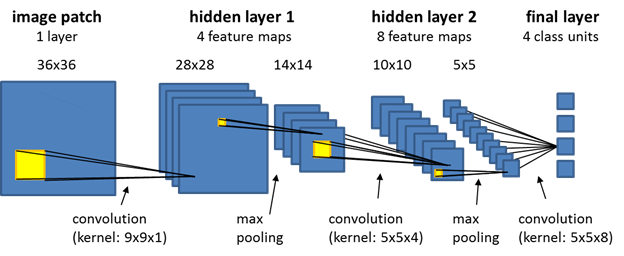
\includegraphics[width=0.49\textwidth]{Fig/1.png}
   \caption{Plot of a schematic structural diagram of a Convolutional Neural Network (CNN). The structure of a simplified CNN, including input layer, hidden layer and output layer can be viewed here.} \label{fig1}
\end{figure}

\subsubsection{The Essence of Convolution}

Central to the concept of CNNs is the convolution operation. This process involves a filter or kernel traversing over an input (like an image) to detect specific patterns. One can envision this as a magnifying glass meticulously scanning a photograph, identifying and registering vital details. The convolution operation is mathematically represented as:

\[ (f * g)(i, j) = \sum_{m} \sum_{n} f(m,n) \cdot g(i-m, j-n) \]

Each coordinate \( (i, j) \) undergoes evaluation, with the resultant observations consolidated in a feature map.

\subsubsection{The Role of the Kernel}

The kernel is a matrix of learnable parameters, typically compact in size. It can be viewed as a pattern template. For grayscale images, common kernel dimensions are \(3 \times 3\) or \(5 \times 5\). As the kernel moves over the input, it employs a uniform weight set, leading to parameter efficiency and an intrinsic capability to discern patterns, regardless of their spatial positioning. Distinct kernels can be analogized as specialized detective tools, each proficient in detecting specific visual nuances, ranging from rudimentary edges to intricate textures.

\subsubsection{Anatomy of a CNN}

A closer inspection of a CNN reveals a sequential arrangement of convolutional layers, punctuated by activation functions such as the ReLU to imbue non-linearity. For enhancing computational efficiency, pooling layers are often interspersed, which, while reducing data dimensions, retain essential information. Progressing deeper into the network, there is an evident shift: from identifying rudimentary patterns to deciphering intricate structures. The culmination typically features fully connected layers, synthesizing the extracted insights for subsequent classification or prediction tasks.

CNNs' distinguishing factor lies in their hierarchical architecture, empowering them to metamorphose raw pixel data into insightful visual interpretations. In stark contrast to traditional computer vision techniques, CNNs obviate the need for manually engineered features, underscoring their adaptability and proficiency across a myriad of challenges and data terrains.

\subsection{Dilated Convolution}

Dilated Convolution, alternatively referred to as Atrous Convolution, introduces a nuanced modification to the conventional convolution operation in neural architectures. Conceptually, it extends the receptive field of convolution without enlarging the kernel itself. This adaptation has proven pivotal, particularly in image segmentation tasks.

\begin{figure}[htbp]
   \centering
   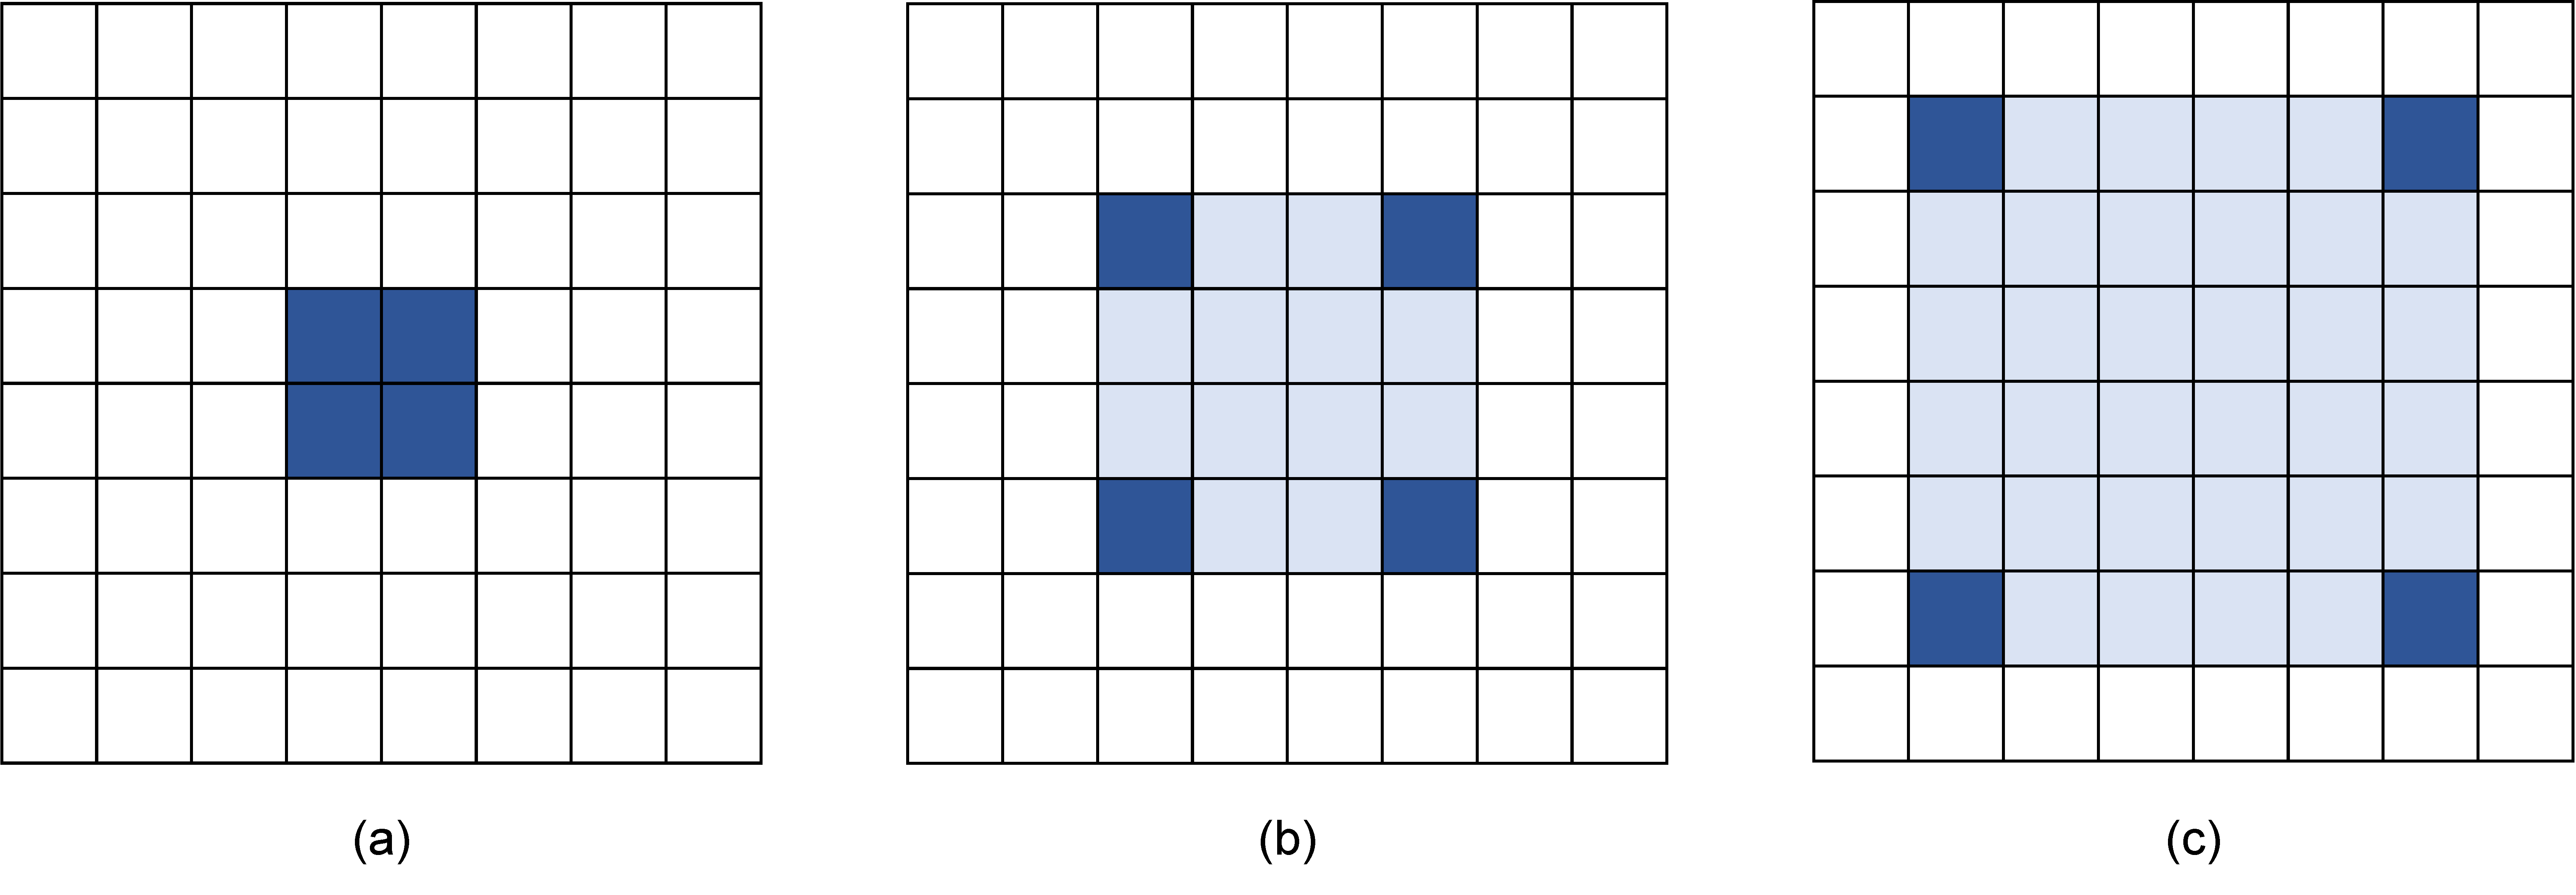
\includegraphics[width=0.48\textwidth]{Fig/2.pdf}
   \caption{Demonstration of dilated (atrous) convolutions with varying dilation rates. In image (a), there is no spacing between blue squares, corresponding to a dilation rate of 1 (standard convolution). Image (b) has a single white square spacing, signifying a rate of 2, while in image (c), two white square spaces yield a dilation rate of 3.}
   \label{fig2}
\end{figure}

\begin{algorithm*}
   \caption{Transformer Model Pseudocode}
   \begin{algorithmic}[1] % The number tells where the line numbering should start
      \Procedure{Transformer}{input, output}
      \State Initialize encoder and decoder parameters
      \State encoder\_output $\gets$ \Call{Encoder}{input}
      \State decoder\_output $\gets$ \Call{Decoder}{encoder\_output, output}
      \State \textbf{return} decoder\_output
      \EndProcedure
      \Statex
      \Procedure{Encoder}{input}
      \State $x \gets \text{input}$
      \For{each layer in encoder\_layers}
      \State $x \gets x + \Call{MultiHeadSelfAttention}{x}$ \Comment{Residual connection}
      \State $x \gets x + \Call{FeedForwardNN}{x}$ \Comment{Residual connection}
      \EndFor
      \State \textbf{return} x
      \EndProcedure
      \Statex
      \Procedure{Decoder}{encoder\_output, output}
      \State $y \gets \text{output}$
      \For{each layer in decoder\_layers}
      \State $y \gets y + \Call{MultiHeadSelfAttention}{y}$ \Comment{Residual connection}
      \State $y \gets y + \Call{MultiHeadCrossAttention}{y, encoder\_output}$ \Comment{Attending to encoder's output}
      \State $y \gets y + \Call{FeedForwardNN}{y}$ \Comment{Residual connection}
      \EndFor
      \State \textbf{return} y
      \EndProcedure
      \Statex
      \Function{MultiHeadSelfAttention}{x}
      \State Split $x$ into $Q$, $K$, $V$ matrices \Comment{Linear transformation}
      \For{$i \in \{1, \ldots, \text{number\_of\_heads}\}$}
      \State $Q_i, K_i, V_i \gets \Call{TransformForHead}{Q, K, V, i}$
      \State $head\_i\_output \gets \Call{Attention}{Q_i, K_i, V_i}$
      \EndFor
      \State $output \gets \Call{Concatenate}{\text{head\_i\_outputs}}$
      \State \textbf{return} output
      \EndFunction
      \Statex
      \Function{Attention}{Q, K, V}
      \State $scores \gets \frac{QK^\top}{\sqrt{d_k}}$
      \State $weights \gets \text{softmax}(scores)$
      \State $output \gets weights V$
      \State \textbf{return} output
      \EndFunction
   \end{algorithmic}
\end{algorithm*}

% \caption{Pseudocode detailing the architecture of the Transformer model, a prevalent neural network structure designed for sequence-oriented tasks within natural language processing. The model integrates both an encoder and a decoder, each composed of multiple layers featuring multi-head self-attention mechanisms and feed-forward neural networks. Specifically within the decoder, a multi-head cross-attention mechanism is implemented to reference the encoder's output. Central to this architecture is the capacity for the model to concurrently emphasize varied segments of the input via the attention mechanisms. Post every sub-layer, residual connections are infused, bolstering both the stability and efficiency during training.}

\subsubsection{The Mechanics Behind Dilated Convolution}

The essence of dilated convolution lies in integrating deliberate intervals or "holes" within the convolution kernel. This procedure effectively broadens the spatial region under the kernel's scrutiny without incurring additional weight parameters. The magnitude of these intervals is stipulated by a dilation rate \( r \). When \( r = 1 \), it replicates the standard convolution. The underlying mathematical representation is:

\[ (f *_{r} g)(i, j) = \sum_{m} \sum_{n} f(m,n) \cdot g(i-r \times m, j-r \times n) \]

\subsubsection{On Kernels and Their Intervals}

Under typical conditions, a \(3 \times 3\) kernel encompasses a \(3 \times 3\) segment of the image. Introducing a dilation rate \( r \) of 2 extends this kernel's coverage to a \(5 \times 5\) region, albeit with intervening gaps. Elevating \( r \) to 3 expands its purview to a \(7 \times 7\) area. Notably, despite this extended field of view, the kernel retains its original weight count.

\subsubsection{Domains Where Dilated Convolution Flourishes}

Though initially conceived for speech signal processing, dilated convolution ascended to prominence within architectures such as DeepLab, tailored for image segmentation. By metaphorical analogy, it equips networks with binoculars, enabling a more extensive contextual view of images without necessitating additional parameters or resorting to data downsampling methods. Employing a diverse ensemble of dilation rates permits the model to simultaneously capture intricate details and overarching patterns. This ingenious augmentation enhances the model's vision without added computational heft. Such advancements have paved the way for unprecedented progress in deep learning, fostering innovations in various vision-related tasks.

\subsection{The Transformer Model}

Introduced in 2017 by Vaswani et al. in their seminal paper "Attention is All You Need", the Transformer model has since emerged as the foundational architecture for many tasks in the realm of natural language processing. Notably, it eschews conventional RNNs and CNNs, relying solely on the self-attention mechanism to discern dependencies within the input data. Such a design facilitates the parallel processing of the entire input sequence, thus optimizing computational efficiency.

\subsubsection{Multi-head Attention Mechanism}

At the heart of the Transformer lies its multi-head self-attention mechanism. In the single-head attention variant, matrices for the query (Q), key (K), and value (V) are constructed from the input. The subsequent attention weights are computed as:
\[ \text{Attention}(Q, K, V) = \text{softmax}\left(\frac{QK^T}{\sqrt{d_k}}\right) V .\]
Here, \(d_k\) represents the dimensionality of the key. This mechanism enables the model to allocate distinct attention weights to various segments of the input.

Extending this, the multi-head attention performs several attention operations concurrently, each relying on unique linear projections. This simultaneous focus on diverse sections and attributes of the input is captured as:
\[ \text{MultiHead}(Q, K, V) = \text{Concat}(\text{head}_1, \dots, \text{head}_h)W_O ,\]
where each \(\text{head}_i\) is:
\[ \text{head}_i = \text{Attention}(QW_{Qi}, KW_{Ki}, VW_{Vi}) .\]
In this formulation, \(W_{Qi}\), \(W_{Ki}\), and \(W_{Vi}\) are weight matrices for each respective head, and \(W_O\) denotes the output weight matrix.

\subsubsection{Architecture of the Transformer}

A canonical Transformer comprises stacked encoders and decoders. The encoder stack entails several replicable encoder layers, each featuring two primary segments: multi-head self-attention and a feed-forward neural network. While the decoder stack mirrors this structure, it introduces an extra multi-head attention layer that centers on the encoder's output. Furthermore, the Transformer integrates residual connections post each sub-layer, and employs layer normalization, ensuring training stability. Training the model follows traditional back-propagation and optimization methodologies.

\begin{figure*}[htbp]
   \centering
   \begin{minipage}[t]{0.33\textwidth}
      \centering
      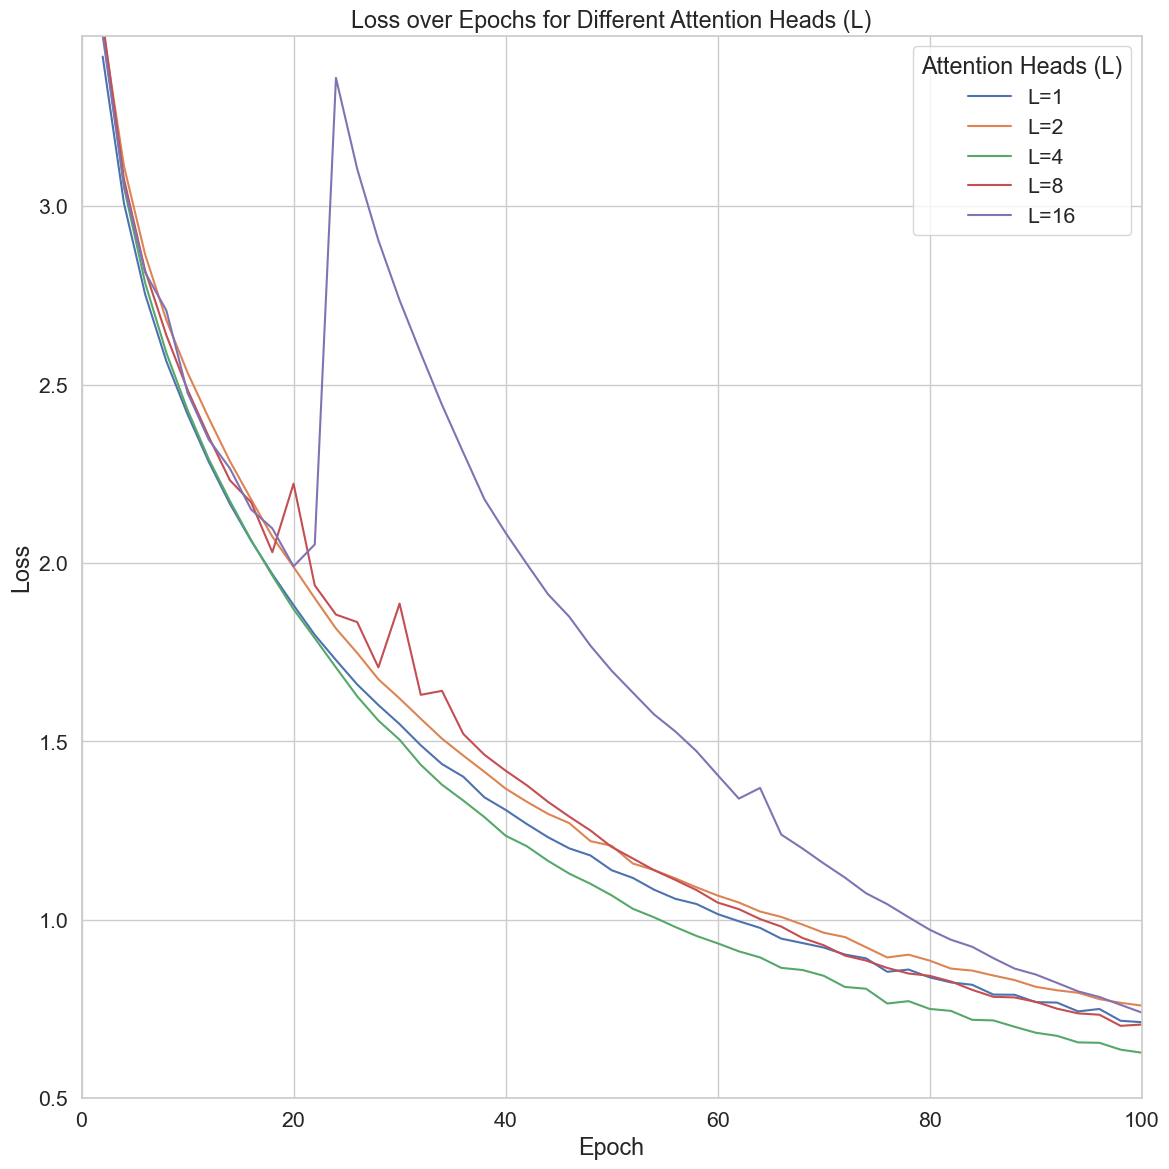
\includegraphics[width=\textwidth]{Fig/3.png}
   \end{minipage}
   \begin{minipage}[t]{0.33\textwidth}
      \centering
      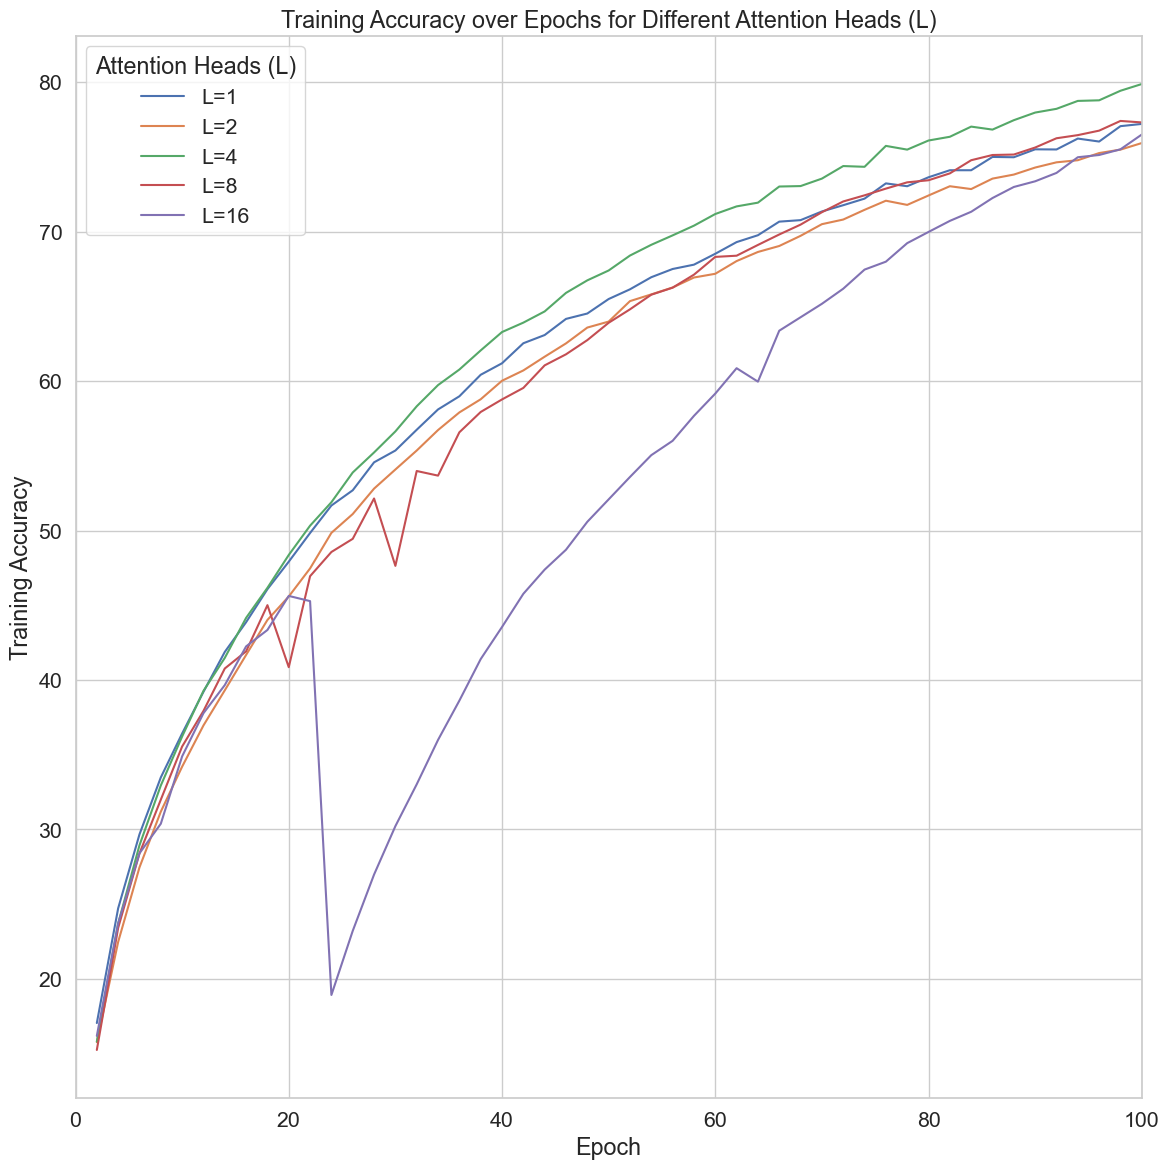
\includegraphics[width=\textwidth]{Fig/4.png}
   \end{minipage}
   \begin{minipage}[t]{0.33\textwidth}
      \centering
      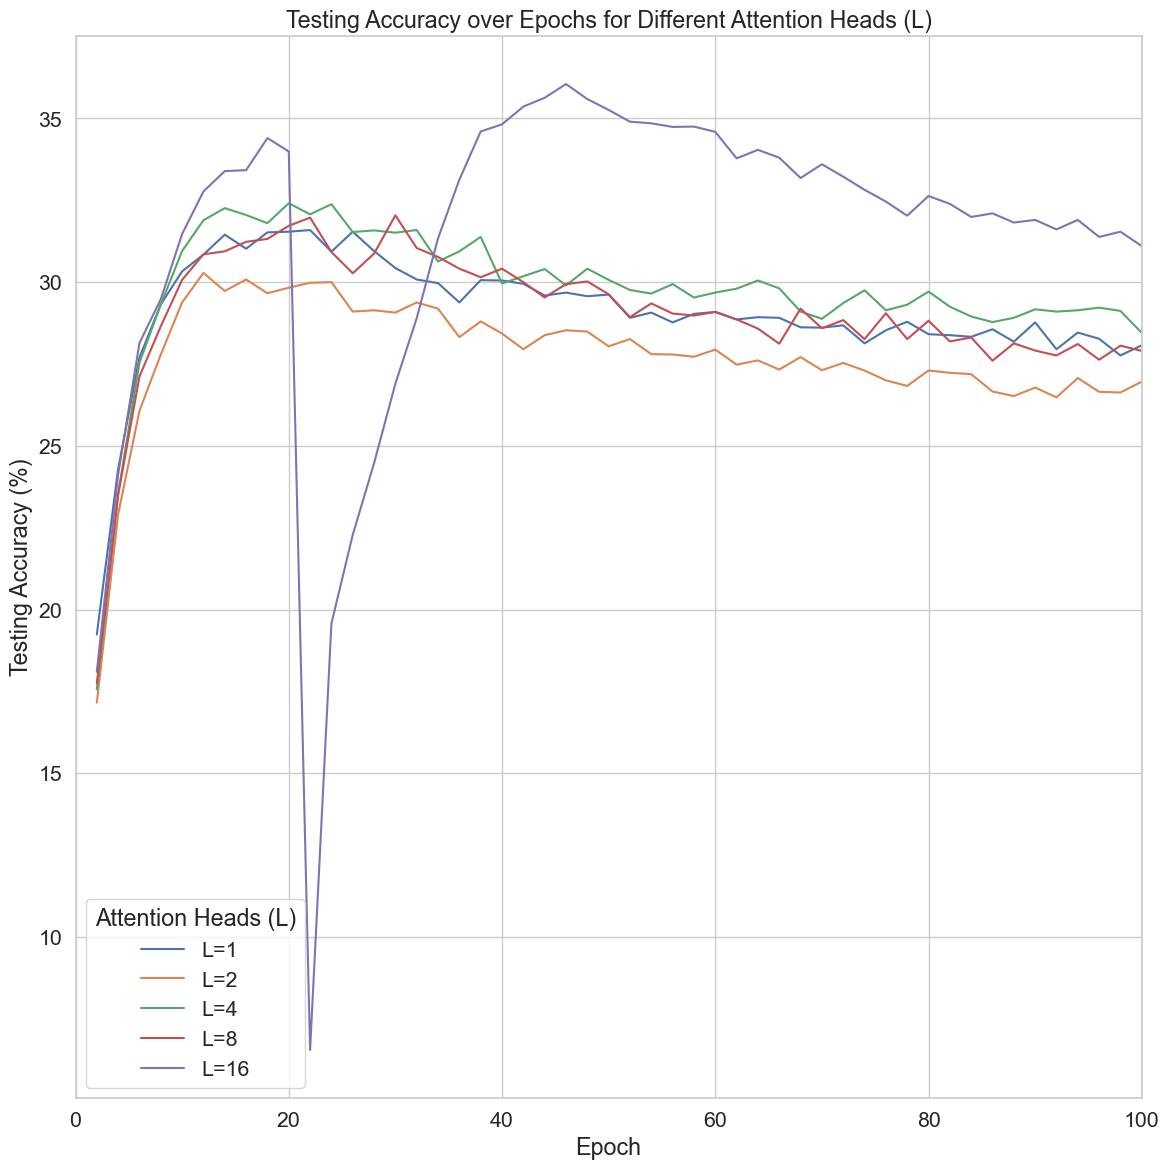
\includegraphics[width=\textwidth]{Fig/5.png}
   \end{minipage}
   \caption{The impact of different attention heads (\(L\)) on model training.}
\end{figure*}

\section{Experimentation} \label{sec:experimentation}

\subsection{Experimentation Environment}

Our experimental setup was built upon a robust computing infrastructure. The central processing unit (CPU) used for this experimentation was dual Intel(R) Xeon(R) CPU E5-2696 v3, with 36 cores and 72 threads. To accelerate the deep learning computations, we employed an NVIDIA GeForce RTX 3090 GPU with CUDA Version 12.2. The system was equipped with a copious memory of 256 GB, ensuring that the most memory-intensive tasks ran smoothly without any resource constraints. On the software front, our system was powered by the Ubuntu 22.04.3 LTS (Jammy) operating system, offering stability and compatibility. The experimentation codes were developed using Python 3.11.5, and all deep learning models were implemented and evaluated using PyTorch 2.1, leveraging its advanced features and optimization capabilities.


\subsection{Data Analysis and Preprocessing}

The CIFAR-100 dataset stands as a renowned benchmark in the computer vision community, encompassing a diverse array of 100 categories with 600 images in each category. This results in a comprehensive set of 60,000 RGB images, each of a resolution of 32x32 pixels. Prior to model training, it is imperative to preprocess these images for optimal model performance. This entails converting pixel values into tensors, thereby presenting the data in a format more amenable to our neural network architectures. To ensure normalization and consistent input distributions, we employed the \texttt{transforms.Normalize} function, adjusting pixel values to lie between -1 and 1. Such preprocessing aids in stabilizing training dynamics.

Model training can be metaphorically related to batch processing in baking. The \texttt{DataLoader} utility allows us to specify the size of these batches using the \texttt{batch\_size} parameter. While it's beneficial to introduce variability in training data to bolster the model's generalization capabilities, we maintained the integrity of the test set to ensure an unbiased evaluation. Regardless of the dataset's format—whether it be numpy arrays or pandas DataFrames—our preprocessing pipeline is designed to be both adaptable and precise, ensuring that any dataset, be it CIFAR-100 or another, can be seamlessly integrated into our training framework.

\subsection{Model Implementation}

The MobileViT architecture is designed to synergistically integrate the strengths of convolutional neural networks (CNNs) and transformers, targeting efficient image classification. This implementation epitomizes the successive advancements in deep learning, and we elucidate its architectural nuances and its distinctions from conventional ViT models.

\textbf{Convolutional Layers:}
A distinguishing characteristic of MobileViT is its astute amalgamation of convolutional layers and transformer blocks. The inception stages of the model utilize convolutional operations. Functions such as \texttt{conv\_1x1\_bn} and \texttt{conv\_nxn\_bn} delineate the convolutional blocks equipped with batch normalization and the SiLU (Sigmoid Linear Unit) activation function. These layers predominantly capture local patterns in images, leveraging the inherent strength of CNNs.

\textbf{Transformer Layers:}
Subsequent to the convolutional phases, the architecture incorporates the transformer framework through the \texttt{Transformer} class. This class is constituted of attention mechanisms (encapsulated in the \texttt{Attention} class) and feed-forward networks (defined within the \texttt{FeedForward} class), with both components ensconced within a \texttt{PreNorm} layer. The attention mechanism is architected using multi-head self-attention, facilitating the model's ability to concentrate on diverse segments of an image concurrently. Given that transformers are adept at discerning global dependencies, their inclusion enables MobileViT to adeptly discern both local and global image patterns.

\textbf{MobileViT Blocks:}
The \texttt{MobileViTBlock} class plays a crucial role in intertwining the convolutional and transformer modules. It orchestrates a sequence of convolutional processes to produce local representations, succeeded by transformer operations that discern global patterns. These local and global features subsequently undergo fusion and further processing, ensuring an exhaustive interpretation of the image content.

\textbf{Depthwise Separable Convolutions:}
A signature feature of MobileViT's efficacy lies in its adoption of depthwise separable convolutions, instantiated within the \texttt{MV2Block} class. Rather than employing conventional convolutions, the architecture opts for a bifurcated approach: an initial depthwise convolution succeeded by a pointwise convolution. This strategy substantially curtails the parameter count while preserving performance, rendering the model more streamlined and apt for mobile platforms.

\textbf{Dynamic Design:}
While the prototypical MobileViT structure remains static, an adaptable variant, named \texttt{DynamicMobileViT}, proffers versatility regarding the count of blocks and channels. Such flexibility ensures the architecture's adaptability to varied computational constraints and application scenarios.

\textbf{Contrasting with Traditional ViT:}
In contrast to the archetypal Vision Transformer (ViT) which segments an image into consistent patches and subsequently applies linear embedding prior to introducing them to a pure transformer structure, MobileViT employs a fusion of convolutional layers and transformers. This hybridized approach addresses the lacunae in ViT's capability to process local features, ensuring a harmonized feature depiction, especially pertinent for images replete with intricate details.

\begin{figure*}[htbp]
   \centering
   \begin{minipage}[t]{0.33\textwidth}
      \centering
      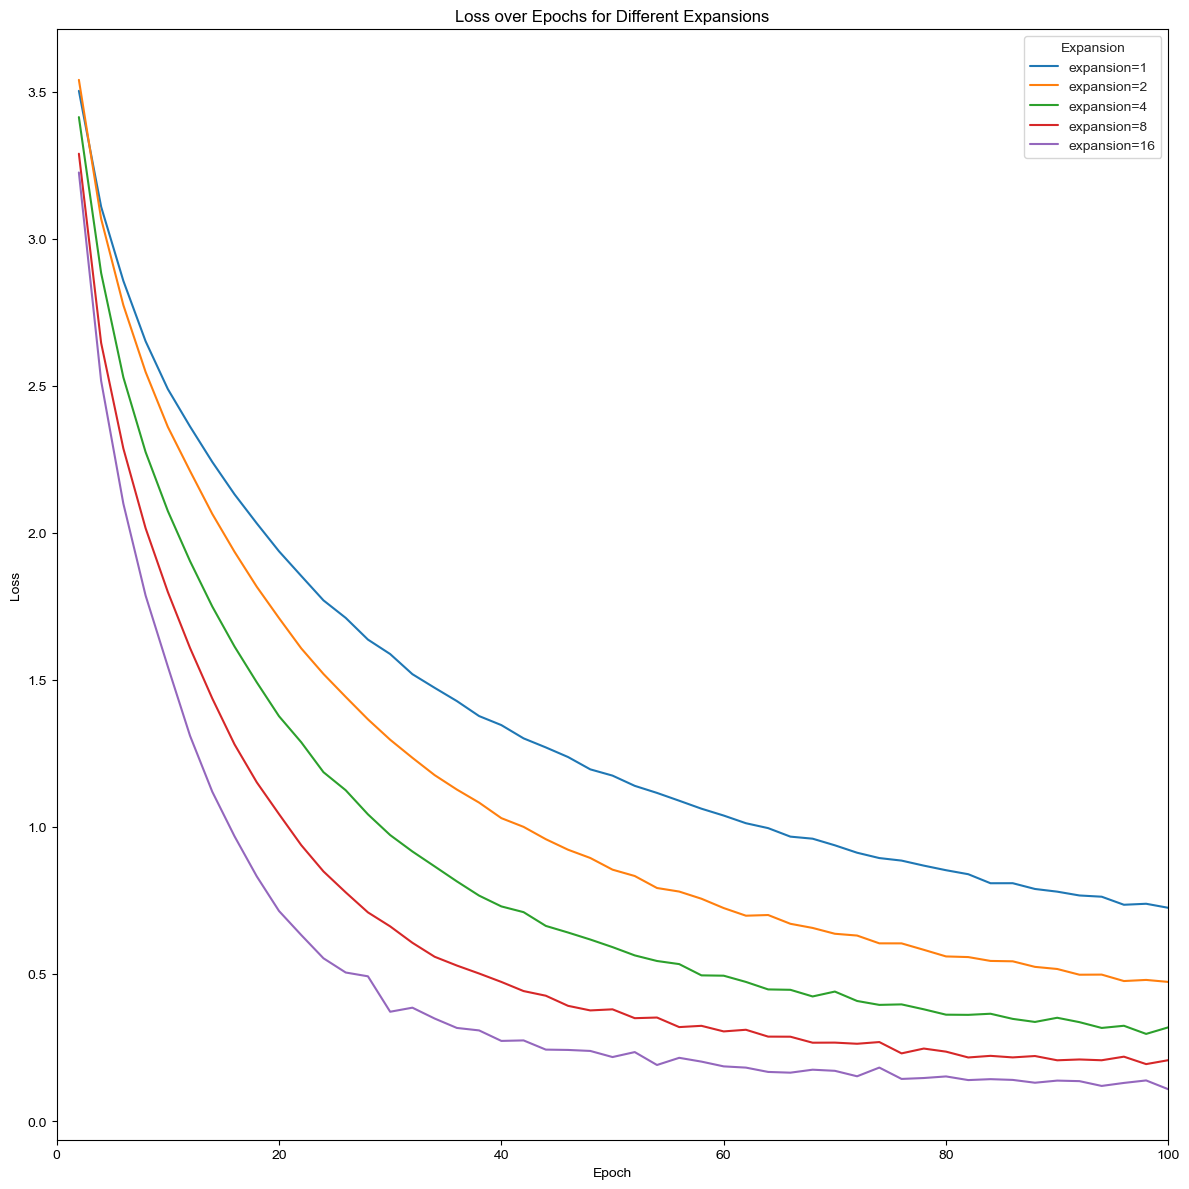
\includegraphics[width=\textwidth]{Fig/6.png}
   \end{minipage}
   \begin{minipage}[t]{0.33\textwidth}
      \centering
      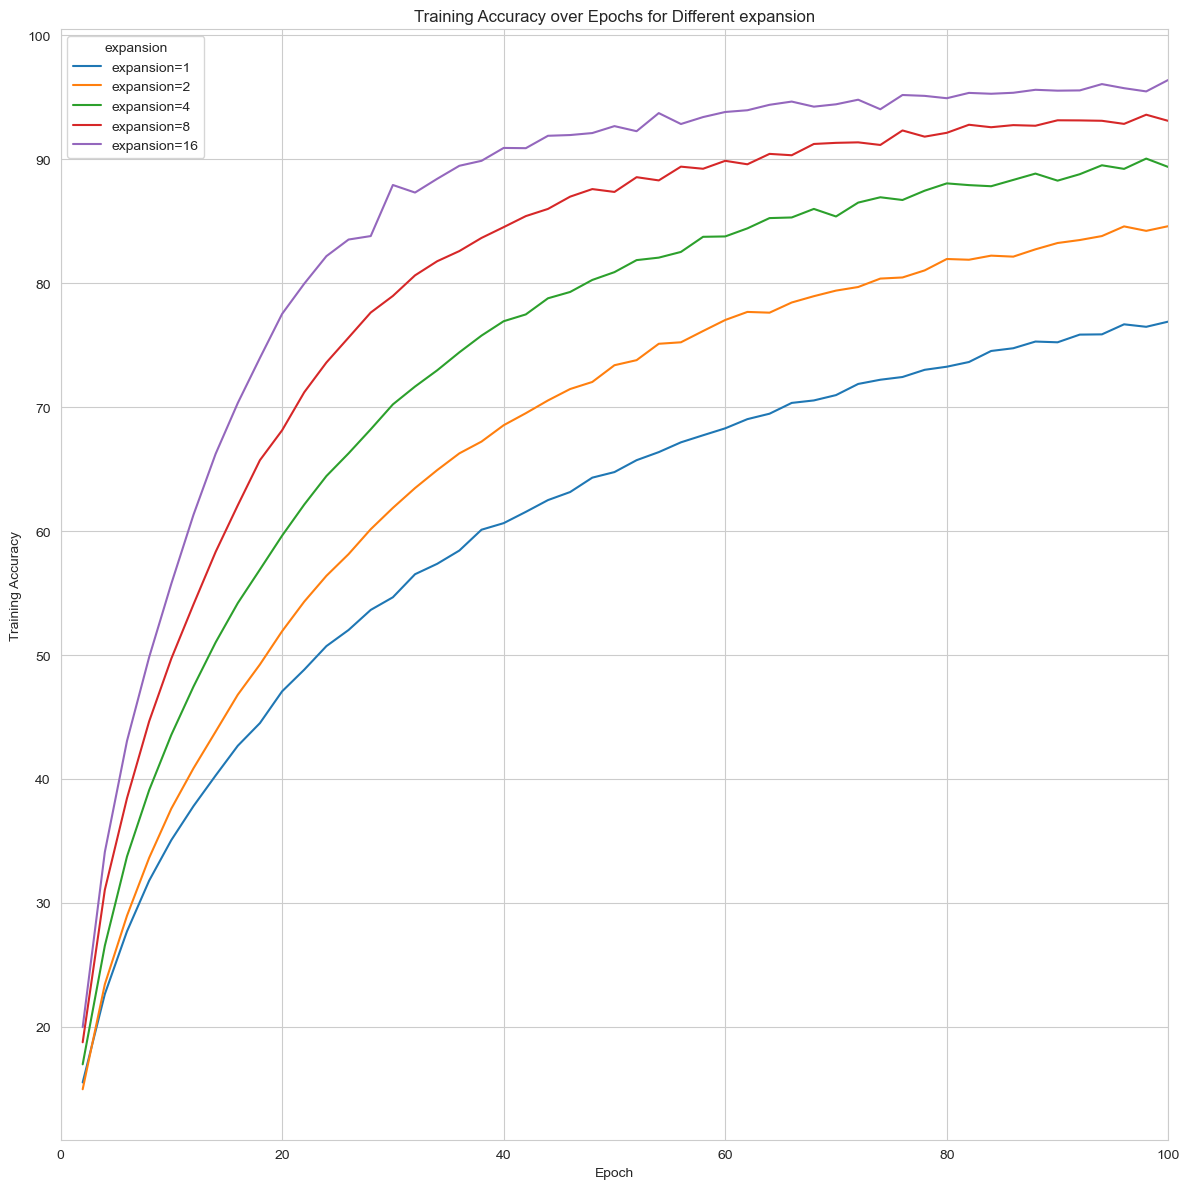
\includegraphics[width=\textwidth]{Fig/7.png}
   \end{minipage}
   \begin{minipage}[t]{0.33\textwidth}
      \centering
      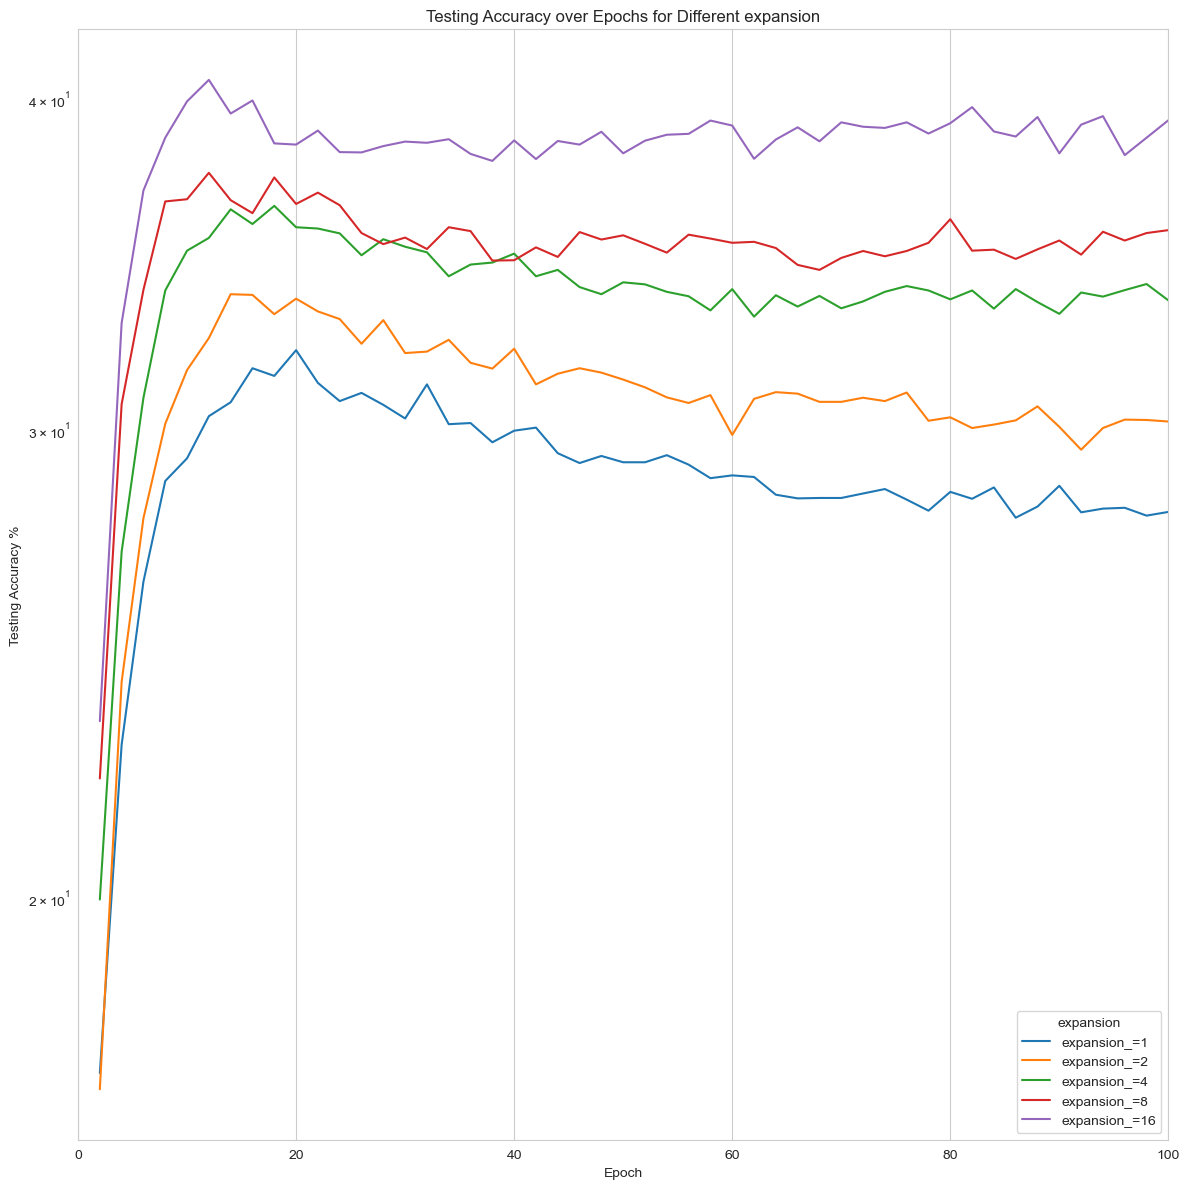
\includegraphics[width=\textwidth]{Fig/8.png}
   \end{minipage}
   \caption{The impact of Different Expansion rates (\(r\)) on model training.}
\end{figure*}

\section{Results} \label{sec:results}

\subsection{Multi-head Attention}

\begin{table}[h!]
   \centering
   \footnotesize
   \begin{tabular}{lccccc}
      \hline
      \textbf{Metric}         & \textbf{L=1} & \textbf{L=2} & \textbf{L=4} & \textbf{L=8} & \textbf{L=16} \\ \hline
      \textbf{Loss}           & 0.7131       & 0.7596       & 0.6276       & 0.7066       & 0.7401        \\
      \textbf{Train Acc (\%)} & 77.22        & 75.94        & 79.89        & 77.32        & 76.51         \\
      \textbf{Test Acc (\%)}  & 28.07        & 26.96        & 28.45        & 27.90        & 31.10         \\
      \textbf{Time (min)}     & 29.14        & 38.53        & 43.37        & 66.90        & 88.52         \\ \hline
   \end{tabular}
   \caption{Metrics of Models with Different Attention Heads (L)}
   \label{tab:performance_metrics_transposed}
\end{table}



The cardinality of attention heads (\(L\)) in a model exerts a significant influence on its performance metrics with the CIFAR-100 dataset. An analysis of the plotted data reveals that an augmentation in the number of attention heads tends to stabilize the training loss. Models equipped with \(L=8\) and \(L=16\) attention heads exhibit a more consistent decrement in loss, which suggests a superior capacity for capturing the intricacies of the dataset. Conversely, the early convergence witnessed in models with \(L=1\) and \(L=2\) might signal an inclination towards overfitting or a diminished ability to generalize across complex patterns.

In the context of training accuracy, a conspicuous decline is observed in the \(L=1\) configuration around the 40-epoch mark, which could be attributed to either instability during the training phase or anomalous data. Models with a greater number of attention heads, such as \(L=8\) and \(L=16\), not only reached higher accuracies but also displayed remarkable stability across the training epochs. This pattern underscores the hypothesis that an increased number of attention heads is potentially more advantageous for managing datasets with a high feature diversity, such as CIFAR-100.

Nevertheless, the definitive gauge of a model's efficacy is its performance on a validation set. The test accuracies for all the models hovered between 30\% to 35\%, indicating a scope for further enhancements. The \(L=1\) model's pronounced dip in accuracy subsequent to the 20th epoch is reflective of its training behavior, thus suggesting an overfitting predicament. In contrast, models with \(L=8\) and \(L=16\) consistently surpassed their counterparts, corroborating the premise that a multitude of attention heads can ameliorate a model's generalization aptitude. In essence, for challenges as formidable as the CIFAR-100 classification task, models with a greater number of attention heads appear to present an optimal synthesis of stability and performance efficacy.

\begin{figure*}[htbp]
   \centering
   \begin{minipage}[t]{0.33\textwidth}
      \centering
      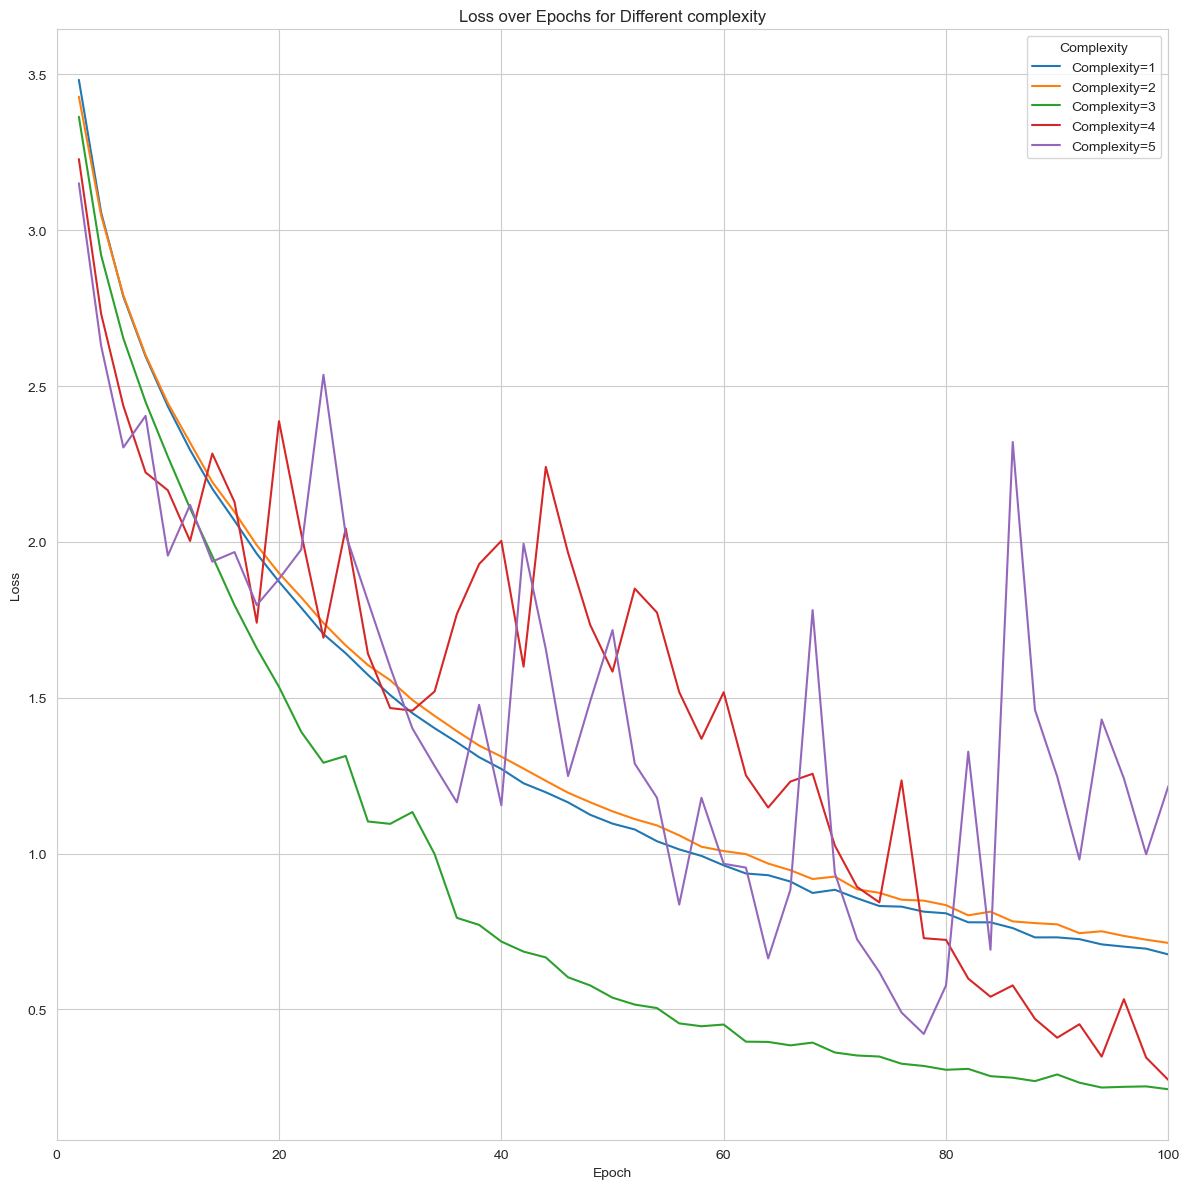
\includegraphics[width=\textwidth]{Fig/12.png}
   \end{minipage}
   \begin{minipage}[t]{0.33\textwidth}
      \centering
      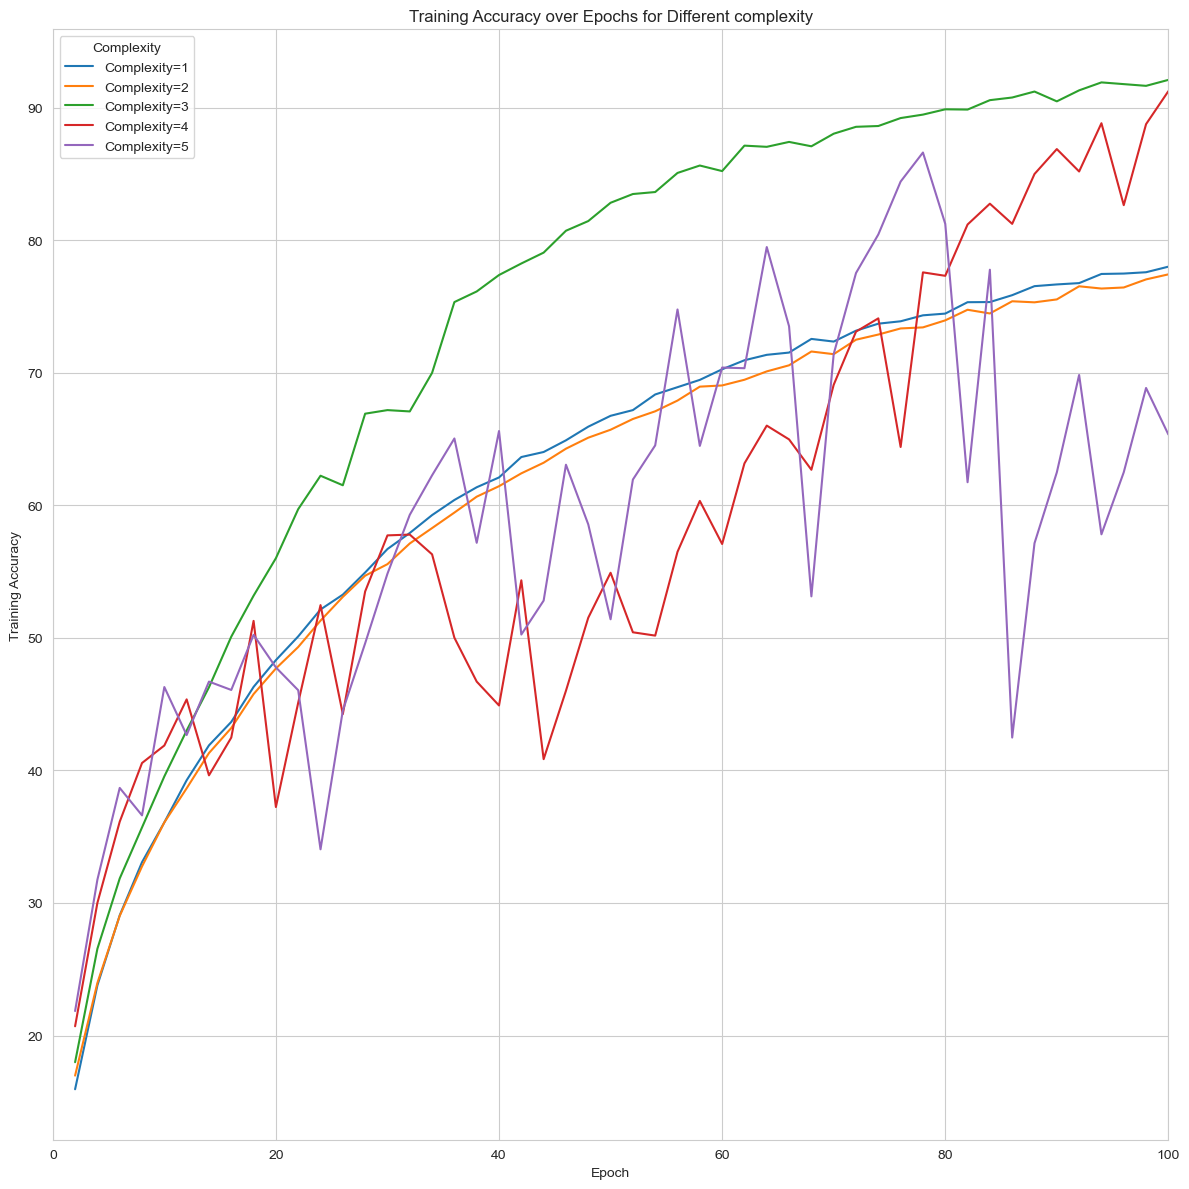
\includegraphics[width=\textwidth]{Fig/13.png}
   \end{minipage}
   \begin{minipage}[t]{0.33\textwidth}
      \centering
      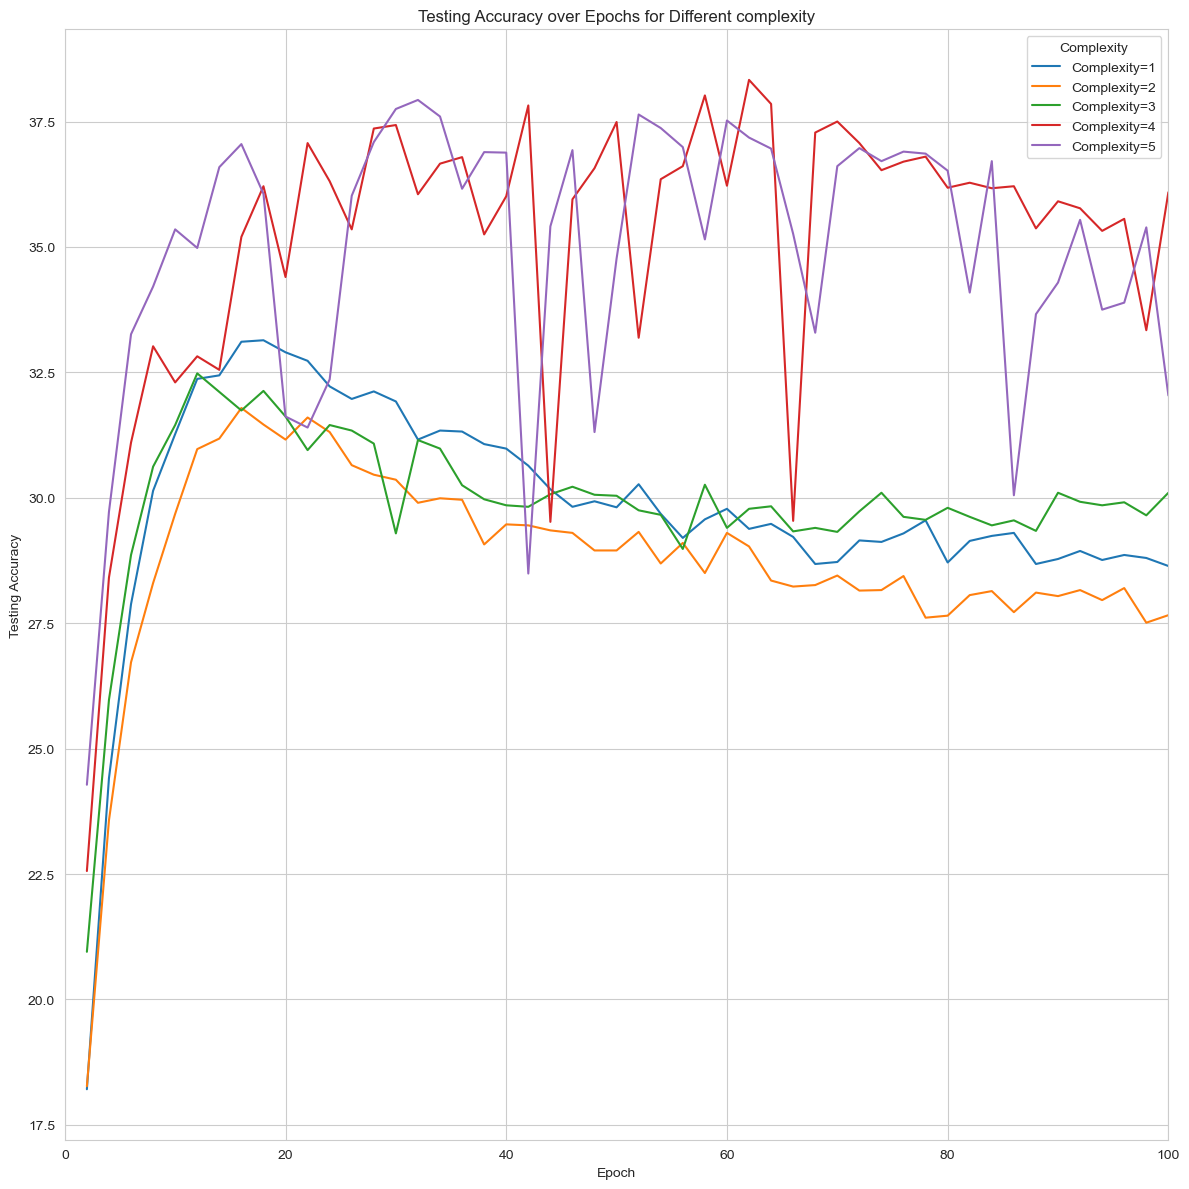
\includegraphics[width=\textwidth]{Fig/14.png}
   \end{minipage}
   \caption{The impact of Different Complex Level on model training.}
\end{figure*}

\subsection{Expansion Rate}

\begin{table}[h!]
   \centering
   \footnotesize
   \begin{tabular}{lccccc}
      \hline
      \textbf{Metric}         & \textbf{r=1} & \textbf{r=2} & \textbf{r=4} & \textbf{r=8} & \textbf{r=16} \\ \hline
      \textbf{Train Acc (\%)} & 76.90        & 84.60        & 89.37        & 93.09        & 96.40         \\
      \textbf{Test Acc (\%)}  & 27.93        & 30.21        & 33.56        & 35.67        & 39.24         \\
      \textbf{Time (min)}     & 36.47        & 41.09        & 37.55        & 45.28        & 43.58         \\ \hline
   \end{tabular}
   \caption{Performance Metrics with Different Expansion Rates}
   \label{tab:expansion_performance_transposed}
\end{table}

The investigation into the effect of various expansion rates on model efficacy, within the context of the CIFAR-100 dataset, has elucidated several insightful trends. In the incipient phase of training, specifically within the initial ten epochs, there is a pronounced acceleration in learning, evidenced by a precipitous reduction in loss and a concomitant ascension in accuracy. The model with an expansion rate of unity exhibits a relative underperformance throughout the training progression, characterized by an elevated loss and a diminished accuracy metric. Conversely, the model boasting an expansion rate of sixteen delineates the most auspicious results, achieving the lowest loss and the highest accuracy during the training phase.

Yet, as the training epoch count advances, a ubiquitous deceleration in the rate of amelioration becomes apparent among the models, signaling an approach towards convergence. Despite the distinguished training performance of models with higher expansion rates, such as sixteen, their competitive edge is significantly abated during the testing phase. Test accuracies for models with augmented expansion rates do not conspicuously surpass their counterparts, insinuating the looming threat of overfitting. This overfitting phenomenon is particularly pronounced in models with elevated expansion rates; they perform with commendable proficiency on training datasets but exhibit shortcomings when exposed to novel test data.

In summation, whilst an escalation in expansion rates can potentiate training performance, it does not invariably portend enhanced generalization capabilities on unseen data. The dichotomy in performance between training and validation phases accentuates the imperative of a comprehensive model evaluation, transcending mere training data metrics. It intimates that the optimization of model performance on the CIFAR-100 dataset necessitates a judicious selection of expansion rates, supplemented with strategies designed to curtail overfitting.

\subsection{Complex Level}

\begin{table}[h!]
   \centering
   \footnotesize
   \begin{tabular}{lccccc}
      \hline
      \textbf{Metric}         & \textbf{C=1} & \textbf{C=2} & \textbf{C=3} & \textbf{C=4} & \textbf{C=5} \\ \hline
      \textbf{Loss}           & 0.6762       & 0.7132       & 0.2436       & 0.2733       & 1.2163       \\
      \textbf{Train Acc (\%)} & 78.00        & 77.42        & 92.09        & 91.24        & 65.34        \\
      \textbf{Test Acc (\%)}  & 28.64        & 27.66        & 30.10        & 36.09        & 32.04        \\
      \textbf{Time (min)}     & 36.62        & 38.96        & 35.71        & 42.80        & 35.93        \\ \hline
   \end{tabular}
   \caption{Performance Metrics for Different Complex Levels}
   \label{tab:complex_level_performance_transposed}
\end{table}


Model complexity plays a pivotal role in determining how a model performs throughout its training process and on unseen data. With varying channels and dimensions, we observe how the architecture's depth and breadth directly impact the model's intricacy. For instance, while models with complexities 1 and 2 share identical parameters, suggesting similar architectures, models of complexities 3 through 5 display progressive growth in channels and dimensions. This progression hints at increasing depth and width in the network, potentially affecting the model's ability to generalize.

Analyzing the loss and accuracy charts, one notices that as the model complexity increases, there's a pronounced fluctuation in the loss values, especially in models with complexities 4 and 5. Such volatility can be an indication of overfitting, where the model might be fitting too closely to the training data nuances. In terms of accuracy, while models of complexities 1 and 2 show a relatively stable but slow-growing performance, models 3 through 5 manifest swifter initial growth. However, they also demonstrate increased variability, especially in later iterations, suggesting that while they might be capturing the training data patterns faster, they might also be susceptible to the pitfalls of heightened intricacy.

Finally, when considering accuracy on a test set, the role of complexity becomes even more pronounced. Early iterations in models, especially with complexities 3 to 5, show rapid accuracy surges. But as iterations progress, there's notable instability in performance, especially in models with higher complexities. While the highest complexity model, complexity 5, achieves the greatest overall accuracy, it also exhibits fluctuations, underscoring the trade-off between model intricacy and its ability to generalize consistently across different data sets.

\section{Summary and Conclusion} \label{sec:summary}

In the course of our research, we embarked upon a comprehensive examination of the factors that bear upon the efficacy of computational models within the CIFAR-100 dataset, focusing specifically on the roles of multi-head attention mechanisms, expansion rates, and overall model complexity. The essence of our inquiry was to unravel the intricate relationships between these elements and their subsequent influence on the model's performance indicators.

Our initial findings reveal that augmenting the number of attention heads, denoted by \( L \), engenders a more stable trajectory of training loss. Models endowed with \( L=8 \) and \( L=16 \) attention heads demonstrated superior performance relative to their counterparts with fewer heads, both in terms of training accuracy and their ability to generalize. These observations suggest that an increased quantum of attention heads may be more aptly suited to capture the complexity inherent in diverse datasets such as CIFAR-100. Moreover, our investigation into expansion rates illuminated the precarious equilibrium between bolstered training performance and the hazard of overfitting. Although models with amplified expansion rates manifested exceptional skill during training, their efficacy waned in the context of unfamiliar test data, indicative of an overfitting tendency. This phenomenon underscores the perennial challenge in machine learning of ensuring robust model generalization, transcending beyond impressive training metrics. Additionally, our scrutiny further extended to the effects of escalating model complexity. As the models expanded in both depth and breadth, marked by an increase in channels and dimensions, we observed a corresponding surge in loss variability. This variability could signal the drawbacks of heightened complexity, leading to overfitting despite the initial swift improvement in accuracy.

Reflecting on our efforts, it becomes evident that our investigations have cast light on the subtle yet profound interplay between model configurations and their operational performance. Nevertheless, the realm of deep learning presents a rich tapestry of uncharted territories for further inquiry. Prospective studies might include fine-tuning the balance between the number of attention heads and model complexity, exploring additional regularization methodologies to mitigate overfitting, or investigating alternative architectures that could exhibit enhanced performance on challenging datasets like CIFAR-100. The path we have journeyed thus far serves merely as an introduction to the extensive prospects available for discovery in the field of deep learning.


   % we~\cite{Authors14b} we.1
   {
      \small
      \bibliographystyle{ieeenat_fullname}
      \bibliography{main}
   }





% WARNING: do not forget to delete the supplementary pages from your submission 
% \input{sec/X_suppl}

\end{document}
